\documentclass{article}
\usepackage{fullpage}
\usepackage{parskip}
\usepackage{titlesec}
\usepackage{xcolor}
\usepackage[colorlinks = true,
            linkcolor = blue,
            urlcolor  = blue,
            citecolor = blue,
            anchorcolor = blue]{hyperref}
\usepackage{apacite}
\usepackage{eso-pic}

\renewenvironment{abstract}
  {{\bfseries\noindent{\large\abstractname}\par\nobreak}}
  {}

\renewenvironment{quote}
  {\begin{tabular}{|p{13cm}}}
  {\end{tabular}}

\titlespacing{\section}{0pt}{*3}{*1}
\titlespacing{\subsection}{0pt}{*2}{*0.5}
\titlespacing{\subsubsection}{0pt}{*1.5}{0pt}

\usepackage{authblk}
\makeatletter
\renewcommand\AB@authnote[1]{\rlap{\textsuperscript{\normalfont#1}}}
\renewcommand\Authsep{,~\,}
\renewcommand\Authands{,~\,and }
\makeatother


\usepackage{graphicx}
\usepackage[space]{grffile}
\usepackage{latexsym}
\usepackage{textcomp}
\usepackage{longtable}
\usepackage{multirow,booktabs}
\usepackage{amsfonts,amsmath,amssymb}
% You can conditionalize code for latexml or normal latex using this.
\newif\iflatexml\latexmlfalse
\providecommand{\tightlist}{\setlength{\itemsep}{0pt}\setlength{\parskip}{0pt}}%

\usepackage[utf8]{inputenc}
\usepackage[english]{babel}
\usepackage{natbib}


\begin{document}

\title{Social attitudes cannot be predicted from federal court decisions and
judge characteristics}


\author[ ]{Will T. Adler}
\author[ ]{Anna Coenen}
\author[ ]{Alexander S. Rich}
\author[ ]{Adviser: Dr. Daniel S. Chen}


\affil[ ]{}
\vspace{-1em}


\date{}
\bibliographystyle{apacite}

\begingroup
\let\center\flushleft
\let\endcenter\endflushleft
\maketitle
\endgroup




\section{Question}\label{question}

Federal US circuit courts often make rulings in areas that are socially
relevant to the American public, such as capital punishment, affirmative
action, or racial discrimination. In this project, we seek to measure
how these rulings may affect Americans' social and political attitudes.
Our goal is to determine whether court rulings tend to move attitudes in
the direction ``intended'' by the ruling or whether rulings tend to move
attitudes in the opposite direction or polarize attitudes. We will focus
on rulings about gender discrimination and their impact on on attitudes
about gender roles.

\section{Datasets}\label{datasets}

To address this question we used two datasets.

First, we used the US General Social Survey (GSS), which is a long
running (1972--) survey on social attitudes and behaviors of US American
citizens \citep{smith2013general}. In addition to social attitudes, the
GSS provides demographic and life-course data about respondents. Each
row represents one respondent.

Second, we used a database of federal appeals court cases that were
decided at the level of circuit courts \citep{sunstein2007judges}. The
cases were separated by issue (e.g.~affirmative action, gender
discrimination, racial discrimination). The federal court system is
divided into 12 circuits, each of which establishes legal precedent for
a group of several states. A circuit court case is decided by a randomly
assigned panel of three judges chosen from the pool of judges appointed
to that circuit. The dataset provides information about the outcome of
each case, which is coded as the number of judges who voted in favor the
outcome that can be considered to be more ``progressive'' (for example,
pro-affirmative action, and against racial or gender discrimination).

Another dataset was used to assign judge characteristics to each case
\cite{eb60c240-7076-4b7f-829d-9b68e9f5494c}. This included, for
instance, the number of panel judges who were female, or who were
appointed by a Democratic president. It also included the average number
of female judges (and other characteristics) in the pool of judges for
that circuit at the time of the ruling.

For our analyses reported below, we focused of the issue of gender
discrimination, and restricted ourselves to court case data pertaining
to that issue. In total, we used 100 cases (one case per row) that were
decided between 1995 and 2004. We chose this subset of cases because it
was the subset that had the longest period of intersection with several
relevant questions on the GSS.


\section{Data preprocessing and independent
variables}\label{data-preprocessing-and-independent-variables}

\subsection{GSS predictors}\label{gss-predictors}

When testing for the impact of course cases in our modeling section
below, we controlled for various demographic variables from the GSS.
Specifically, we used the following variables as predictors in our
model(s).

\begin{itemize}
\tightlist
\item
  age (years)
\item
  sex (male; female)
\item
  education (years)
\item
  race (black; white; other)
\item
  region (New England; Middle Atlantic; Mountain; Pacific; South
  Atlantic; East-North Central; East-South Central; West-North Central;
  West-South Central)
\item
  religion (Buddhist; Catholic; Christian; Hindu;
  inter/nondenominational; Jewish; Muslim; Native American; Orthodox
  Christian; Protestant; Other Eastern; Other; None)
\end{itemize}

For discrete predictors, we used one-hot encoding. Continuous variables
were standardized to have zero mean and unit variance. Along with these
predictors, we also included race-by-region and race-by-religion
interactions, and interactions of all demographic predictors with year
in which the survey was administered.

\subsection{Court case predictors}\label{court-case-predictors}

For each case, we computed the difference between the judge ideology on
a given panel and its expected value. To calculate this, we took the
proportion of judges who were appointed by Democratic presidents on each
panel, and subtracted the expected proportion based on the overall pool
of judges in the circuit at the time of the case.

We then grouped court cases by circuit and year, and aggregated them in
different temporal time windows ranging from 1 to 10 years. For each
time window and each circuit we computed the \emph{number of liberal}
and the \emph{number of conservative decisions}, as well as the summed
\emph{difference of judge ideology from expectation} value described
above.

\subsection{Integrating the data
sources}\label{integrating-the-data-sources}

We removed GSS data for years in which court data was unavailable, and
merged the three court predictors with the GSS demographics predictors
by year and circuit (the ``circuit'' of a GSS respondent was determined
by the region they resided in). For each court predictor, we added
interactions of court-predictor-by-year, and
court-predictor-by-demographic for each demographic variable.


\section{Dependent variable: Index of conservative attitudes about
gender
roles}\label{dependent-variable-index-of-conservative-attitudes-about-gender-roles}

\subsection{Approach}\label{approach}

Our dependent variable was people's attitudes towards gender roles. To
operationalize these attitudes, we used 7 questions from the GSS that
asked for people's opinions on gender roles (see below). To arrive at a
single outcome measure, we performed a Principal Components Analysis
(PCA) as a method of dimensionality reduction. Before fitting the PCA,
we standardized the answers to each question to have variance of 1 and
mean of 0. To handle missing data, we excluded every respondent who
answered only four or fewer of the 7 questions. Otherwise, missing
values were imputed using the average response to a given question by
other respondents in the same year.

PCA performs a total least squares regression on a number of variables
to find the dimensions that can explain the most (or least) amount of
variance in the data. Each principle component is an eigenvector of the
data's covariance matrix (\(D^TD\)) and the amount of variance
it explains is the corresponding eigenvalue.

\subsection{Resulting measure}\label{resulting-measure}

The first principle component of the 7 gender questions from the GSS
explained 36\% of the variance in the data and by examining its
coefficients for each question, we confirmed that it captures
respondents' level of conservatism regarding gender roles. The following
table summarizes the coefficients per question.

\begin{longtable}[c]{@{}ll@{}}
\toprule
\begin{minipage}[b]{0.6\columnwidth}\raggedright\strut
GSS Statement
\strut\end{minipage} &
\begin{minipage}[b]{0.2\columnwidth}\raggedright\strut
Coefficient of 
\newline
1st principal 
\newline
component
\strut\end{minipage}\tabularnewline
\midrule
\endhead
\begin{minipage}[t]{0.6\columnwidth}\raggedright\strut
A working mother can establish just as warm and secure a relationship
with her children as a mother who does not work.
\strut\end{minipage} &
\begin{minipage}[t]{0.2\columnwidth}\raggedright\strut
-0.53
\strut\end{minipage}\tabularnewline
\begin{minipage}[t]{0.6\columnwidth}\raggedright\strut
Because of past discrimination, employers should make special efforts to
hire and promote qualified women.
\strut\end{minipage} &
\begin{minipage}[t]{0.2\columnwidth}\raggedright\strut
-0.02
\strut\end{minipage}\tabularnewline
\begin{minipage}[t]{0.6\columnwidth}\raggedright\strut
I favor the preferential hiring and promotion of women.
\strut\end{minipage} &
\begin{minipage}[t]{0.2\columnwidth}\raggedright\strut
0
\strut\end{minipage}\tabularnewline
\begin{minipage}[t]{0.6\columnwidth}\raggedright\strut
Most men are better suited emotionally for politics than are most women.
\strut\end{minipage} &
\begin{minipage}[t]{0.2\columnwidth}\raggedright\strut
0.3
\strut\end{minipage}\tabularnewline
\begin{minipage}[t]{0.6\columnwidth}\raggedright\strut
It is much better for everyone involved if the man is the achiever
outside the home and the woman takes care of the home and family.
\strut\end{minipage} &
\begin{minipage}[t]{0.2\columnwidth}\raggedright\strut
0.54
\strut\end{minipage}\tabularnewline
\begin{minipage}[t]{0.6\columnwidth}\raggedright\strut
Family life often suffers because men concentrate too much on their
work.
\strut\end{minipage} &
\begin{minipage}[t]{0.2\columnwidth}\raggedright\strut
0.54
\strut\end{minipage}\tabularnewline
\begin{minipage}[t]{0.6\columnwidth}\raggedright\strut
A preschool child is likely to suffer if his or her mother works.
\strut\end{minipage} &
\begin{minipage}[t]{0.2\columnwidth}\raggedright\strut
0.56
\strut\end{minipage}\tabularnewline
\bottomrule
\end{longtable}

 After projecting the question data on this component, participants with
more traditional views on gender roles (assigning more domestic
responsibilities to women and more professional ones to men) end up with
higher values than more progressive respondents. In the rest of this
report we will use this measure as our dependent variable, which we
refer to as the \emph{gender conservatism index}.


\begin{figure}[h!]
\begin{center}
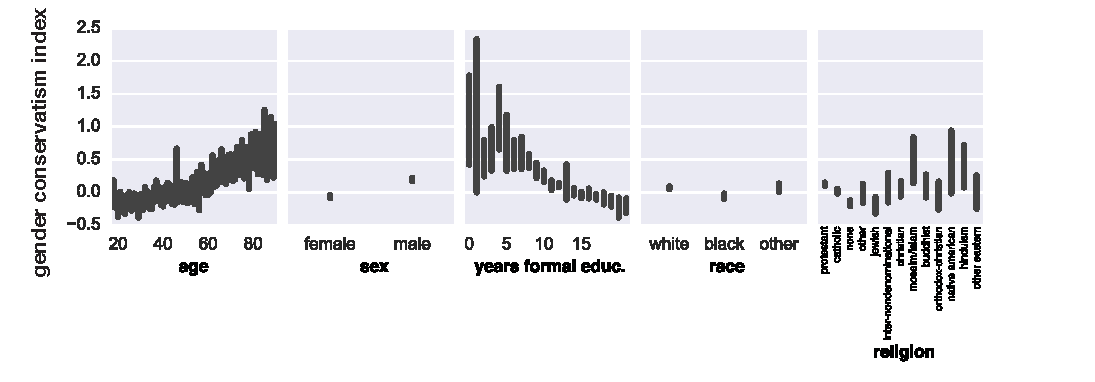
\includegraphics[width=0.7\columnwidth]{figures/gci/gci}
\caption{GSS respondents who were older, male, or had fewer years of
formal education scored highly on the gender conservatism index. Error
bars represent 95\% confidence intervals on the bootstrapped mean.%
}
\end{center}
\end{figure}

\section{Modeling approach}\label{modeling-approach}

\subsection{Main model}\label{main-model}

Our main challenge in modeling these data was to strike a balance
between predictive accuracy and interpretability. On the one hand, we
wanted to make sure that our model was not overfitting the data and made
good predictions. On the other hand, the question of this project
required us to use a method that allowed us to draw inferences about the
impact of specific predictors.

To make sure the results were easy to interpret, we chose to model the
data using linear regression. To make sure our model does not overfit,
we regularized it using L1 regularization (proportion=.9) and L2
regularization (proportion=.1). This elastic net approach gave us the
benefit of sparsity of the solution (due to L1 regularization), while
stabilizing our estimates from correlated predictors via a small amount
of L2 regularization. We chose the total amount of regularization using
10-fold cross-validation within the training set and chose the value
that yielded the lowest average error.

\subsection{Alternative models}\label{alternative-models}

In addition to the regularized linear regression, we also tried a number
of other machine learning algorithms to model our data. Each of these
approaches yielded similar results as our main analysis regarding the
impact of court predictors. Since their outcomes are more difficult to
interpret, we chose to present results only from the linear regression.

Specifically, we tried the following algorithms.

\begin{itemize}
\tightlist
\item
  regression with a decision tree
\item
  regression with a random forest
\item
  regression with AdaBoost
\end{itemize}

In all cases, court-related predictors decreased performance on the
validation set.


\section{Results}\label{results}

All results reported below are calculated based on ten runs of the
model, using a different randomly selected 10\% of the GSS data held out
as a test set on each run.

\subsection{Null model: Demographics
only}\label{null-model-demographics-only}

When predicting the gender conservatism index using demographic
predictors alone, we achieved an \(R^2\) of
\textasciitilde{}.11 on the training set, and \textasciitilde{}.092 on
the test set.

\subsection{Full model: Demographics and court
data}\label{full-model-demographics-and-court-data}

We tested two versions of the full model that included the court data in
addition to demographic predictors. First, we tested a model with court
decisions (no. of conservative/liberal decisions) over different time
windows along with the judge ideology predictor (difference from
expectation in each time window). Second, we also tested a model with
only the judge ideology predictor. Since judges are randomly chosen from
a large pool, their impact on attitudes counts as an interesting
``natural experiment.''

Across all temporal windows tested (1 to 10 years), the addition of
information from recent circuit court decisions did not improve the
prediction of gender conservatism in our test set. This is illustrated
by Figure 2, which shows the \(R^2\) by model type
(demographics only or demographics + court), time window, and dataset
(training or test). On the test set, the full models' performance is
consistently worse than those of the null model.

Although we were unable to detect any impact from the court decisions on
the gender conservatism index, a number of demographic variables proved
reliably predictive of gender conservatism. As Figure 3 shows, among the
most reliable predictors were age, gender, race, education, and religion
of the respondent.


\begin{figure}[h!]
\begin{center}
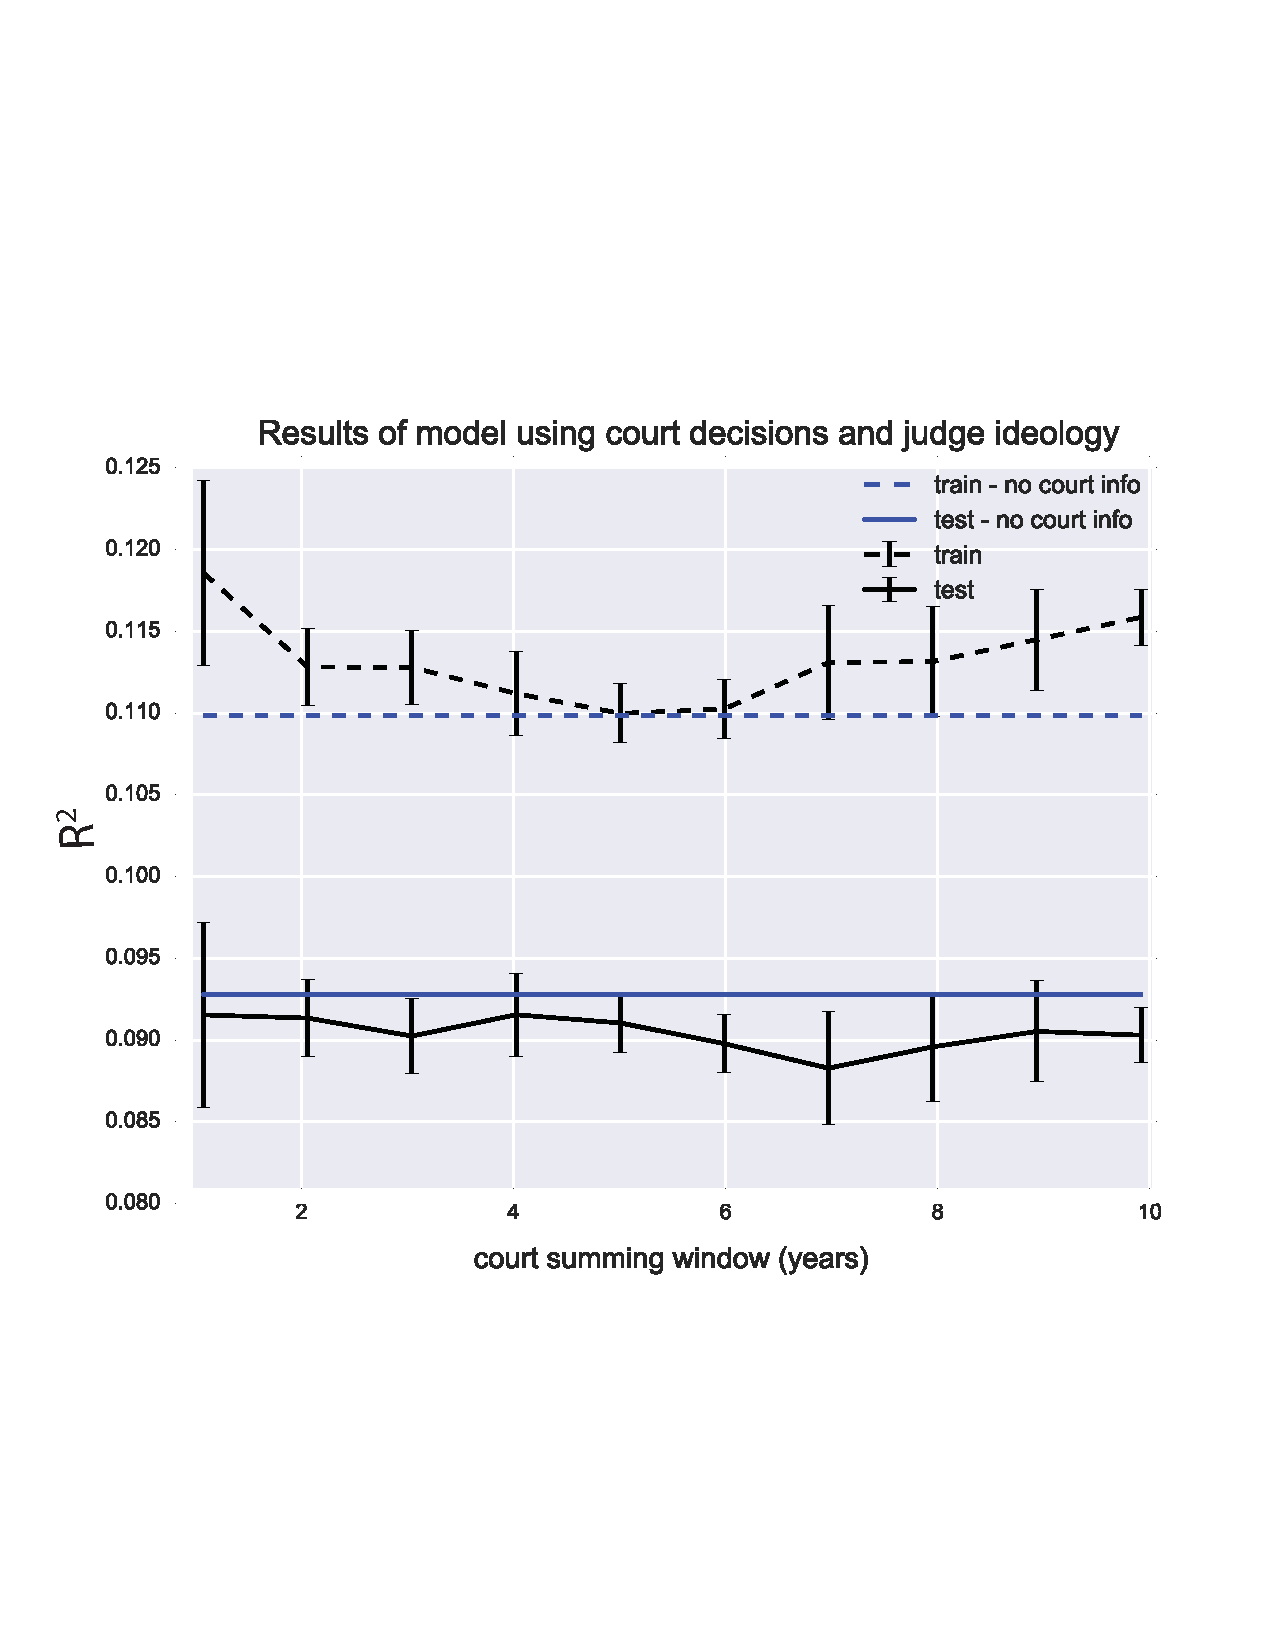
\includegraphics[width=0.7\columnwidth]{figures/summing_windows/summing_windows}
\caption{\(R^2\) of null model (no court) and full model on
training and test set, by court data summing window.%
}
\end{center}
\end{figure}

\begin{figure}[h!]
\begin{center}
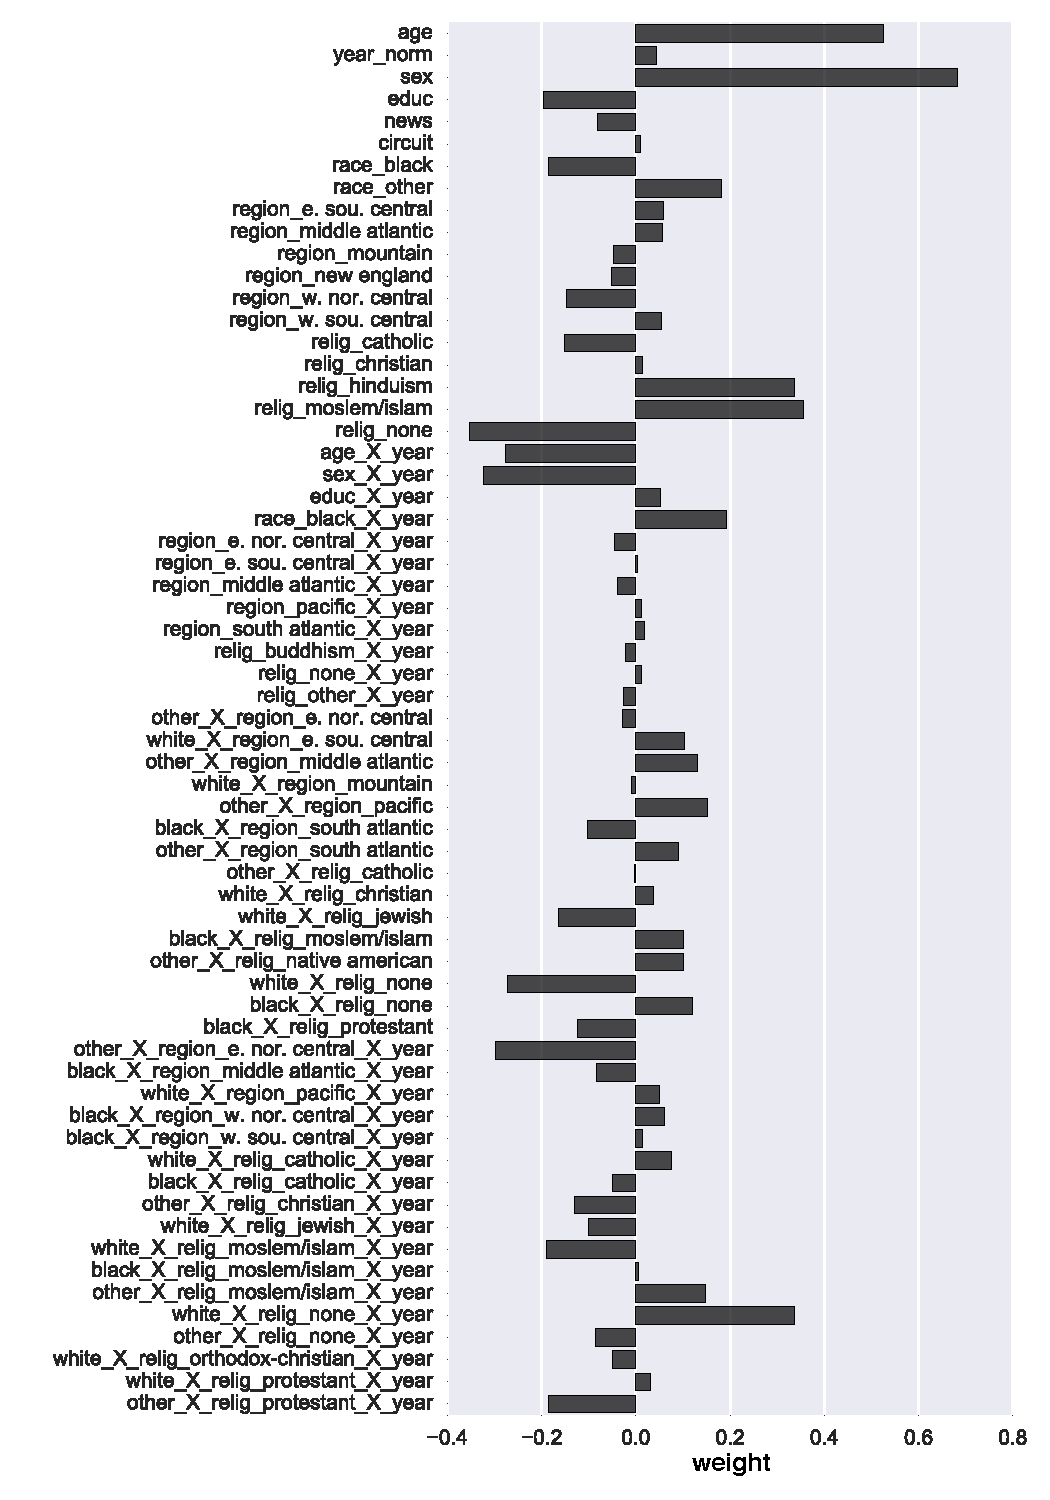
\includegraphics[width=0.7\columnwidth]{figures/coefficients_nocourt1/coefficients_nocourt.pdf}
\caption{GSS demographic predictors of conservative attitudes about
gender roles, from a linear regression model using only demographic
predictors from the GSS (and no court data).%
}
\end{center}
\end{figure}

\section{Discussion}\label{discussion}

Although we used several modeling approaches, we did not find a
relationship between federal court rulings dealing with gender
discrimination and societal attitudes about gender roles. It may be that
most circuit court cases do not reach the public consciousness enough or
are not impactful enough to affect attitudes. Alternatively, it is
possible that cases in another domain such as affirmative action or the
death penalty have a more direct effect on attitudes. Unfortunately, in
many domains our current data set did contain sufficient temporal
overlap between court cases and relevant GSS questions for a
well-powered analysis.

An interesting future direction might be to study this question using
supreme court cases, which (sometimes) receive far greater media
coverage. For example, did the recent Obergefell v. Hodges ruling alter
Americans' views about same-sex marriage? This kind of high-profile case
may be the most likely to shift attitudes perceptibly, though this very
landmark status also means that such cases are rare, and thus difficult
to statistically analyze.

\bibliography{converted_to_latex}


\end{document}

